\documentclass{article}
\usepackage[utf8]{inputenc}

\title{Term Paper ECS 132 Group 22}
\author{Nathan Kim, Grayson Cox, Derek Lin }
\date{March 18 2021}

\usepackage{listings} % inserting code
\usepackage{hyperref}
\usepackage{pdfpages}



\begin{document}


\maketitle



\section{Part A}
    
    \centerline{Use of P-Values as an Indicator of Intent to Vaccinate} 
	\indent Professor Jeanette B. Ruiz analysed public polling which indicated that the intent to vaccinate once COVID-19 vaccines become available will be sub optimal. The sample consisted of 804, English-speaking adults residing in the United States. There were many measures used to appraise COVID-19 vaccine intentions. One interesting relationship that was explored was the effects of Media and Politics on vaccination intentions. Using their own model, it was determined that respondents relying on conservative news sources had a lower intent to vaccinate compared to their democratic counterparts. Following up, the researchers came to the conclusion that all things equal, Republicans were significantly more likely to accept vaccine conspiracies compared to their Independent counterparts. With the researcher’s scoring, the Republican mean acceptance was 2.82 while the Independent mean acceptance was 2.51. This is hardly significant. Given only the p-values and the statement, one can be led to believe there was a whole digit difference between the two parties’ mean acceptance. It would be far more insightful to say that there is a 95\% chance that Republican’s mean acceptance is in between (2.673, 2.967) and that there is a 95\% chance that the true Independent mean acceptance is in between (2.384, 2.636). There is no question regarding the probable magnitude between the two acceptances, and there would be no deceptions with calling this difference significant. A possible ramification would be if the CDC were to use this information to decide who to target to knock down vaccine conspiracies. Being told that there is a significant difference between Republican and Independent acceptance could lead to an insensible focus on the Republican populace when Independents could have used a similar amount of focus. This could significantly hinder progress at developing herd immunity towards COVID-19. Using a p-value strips away important information, and leaves too much to the dictionary definition of significant. Providing a confidence interval instead leaves no guesswork to the individual receiving the statistical analysis.
    -Nathan Kim
    \\
    \href{https://www.ncbi.nlm.nih.gov/pmc/articles/PMC7794597/?fbclid=IwAR24aHyyKyUiKOV1kRIFDTCrim32KTttaLupR1Hhz3U7cvR2dwUcAOa3es0}{\textit{Source Link}}


    \centerline{Validity of P-Tests as an Approach to Sediment Toxicity Testing}
    \indent In the Journal of Environmental Toxicology and Chemistry, Volume 20, Issue 2, Bryn M. Phillips et al. determine threshold toxicity values for sediment (dirt, rocks, etc. underwater). In their assessment, they establish that a sediment sample is to be considered toxic if two criteria are met. The first is that there is a significant difference in organism survival with p < 0.05 between the sample and a negative laboratory control. In addition, they required the difference in organism survival rates to be greater than a 90th percentile minimum significant difference. However, this protocol has significant issues in it's analytical methodology. When taking this into consideration, the first problem that arises is that just because a sediment sample does not significantly change the survival rate does not mean that it does not actually change the survival rate- it very well might, but it might not be represented as significant in that sample. It also fails to include confidence intervals for these toxicity thresholds, which would imply that toxic sediment may not be cleaned up just because it doesn't match with the threshold they calculate (even though some samples under the threshold may well still be toxic). The more samples that they take in, the larger number of erroneous conclusions that will be reached as there is a 5 percent chance of misclassifying non-toxic samples as toxic, and toxic samples as non-toxic. So out of a thousand samples, if 950 of them were actually non-toxic, on average 47.5 would be classified wrongly as toxic. Out of the ones that actually are toxic, on average 2.5 of the samples would be misclassified as non-toxic. Ideally, you would want to consider a looser boundary for a significance test in this case, as the consequences are more severe for mistaking a toxic sample as non-toxic, while confusing a non-toxic sample with a toxic sample would not be quite as bad. However, as establishing this as a threshold for other studies, this is even worse because it does not inform users of the threshold that it might not detect toxic samples as a "significant" result. It's very important to consider that false negative results are worse than false positives. The lack of a lower confidence interval gets rid of the valuable information that the sample might actually be close to the threshold value, but you don't know that because it's all based on a significance test.
    - Grayson Cox 
    \\
    \href{https://setac.onlinelibrary.wiley.com/doi/full/10.1002/etc.5620200218?casa_token=jjDz7jm0-8cAAAAA\%3AkYSAWfP5aaMoDQPezOYtDqe961eoOYyo0DPda7BSMkPPULjZyfcERBB0POyrtg8sztZhKgSAY-kyK6ZE}{\textit{Source Link}}
    
    \centerline{Validity of Significance Testing on the Analysis of Software Development}
    \indent In the 2013 35th International conference on Software Engineering (ICSE), Professor Raisa D’Souza et al. assess the quality of software development within software developer groups based on measurements of focus. Overall results indicate that focus is highly correlated with fewer defects. Files that receive less narrowly focused attention are more likely to contain defects than those from a broader base of contributors. \\
    \indent A recurring theme within open-source software (OSS), is the need for software quality, usually attributed with low defects; however, methods for quantifying software quality has been difficult to perform. Usually, module ownership is attributed to software quality. If a module has many contributors or low ownership, code quality can be adversely impacted. Professor D’Souza et al.’s ecology metaphor of predatory food webs to measure developer and module attention focus. A module is defined to be a file, package, or component, that the developers focus on. Modules are predators, which feed upon the cognitive resources of developers. The more diverse the module is, the more prey that the module eats from. Like diversity in ecology, software development also depends on diversity. Having too high of a diversity is detrimental while having too little diversity is also detrimental. Having the right amount of prey for the predator is good for the ecosystem to thrive.
    \\ \indent There are threats to validity within the experiment. One threat is that complex files do get more defects due to the sheer volume and larger room for error. A method to analyze number of defects proportional to the size of the modules and number of developers could be a plausible choice to eliminate any source of errors. This has potential to skew data because the researchers chose to measure software quality based the number of total defects. Thus, it would serve to be more illuminating to dole out or partition the large data sets into smaller ones to more accurately parse the data. 
    \\ \indent Another threat to validity is the use of significance testing rather than confidence intervals. Professor D’Souza et al. argue that “increased ownership is negatively correlated with defects which is in agreement with previous results, however, is not significant at the 5 percent level.” The term “significant” in this case is actually arbitrary. Since we do not know the number of defects in the study, only that there are some defects or none at all, we do not have valuable information to gauge precise results from data. When these hypotheses are tested, there are chances of false positives as well as false negatives. While hypothesis testing finds that the criteria of the null hypothesis is not met, this does not mean there are insignificant findings in the experiment. On the flip side, if there are null hypothesis is failed to be rejected, this does not conclude that there are significant findings in the experiment. In Professor D’Souza et al.’s experiment, it led to findings that were significant at the 95 percent level. However, because of the misconception of significant testing means these findings were actually not significant. Using confidence intervals to show the range of plausible values is a better practice to avoid data that could be misconstrued as significant or insignificant when it is not. In conclusion, using confidence intervals gives valuable information about the likely magnitude of the effect being investigated and the reliability of the estimate, which significance testing fails to do. -Derek Lin
    \\
    \href{https://citeseerx.ist.psu.edu/viewdoc/download?doi=10.1.1.303.4662&rep=rep1&type=pdf}{\textit{Source Link}}

\section{Part B Disclaimer}
\indent In order to accommodate long run times from the large Porto Taxi data set, accumulating over 171062 instances over a year by 442 Porto Taxi drivers, we used a fixed sample size rather than using the entire data set given. Because of this, our data used in our explanations may differ from other tests run in different instances.

\section{Part B Task 1}
\indent To find patterns within the trip duration, we calculated expected value, variance, coefficient of variation, standard deviation, margin of error, and 95 percent confidence intervals to indicate the average times that individuals used for each trip withstanding variability from a large sample size of 50,000 trips. Plotting the frequency with the frequency times using the hist() function, we found that the shape of the histogram resembled the beta and gamma distributions. However, after testing many different parameters, we came to the conclusion that the beta distribution did not fit our data, while the gamma fit it closely (but with more variation than was in our data). For the trip times, we saw sharp exponential increases towards the peak of the histogram and then from the peak of the histogram, when the slope changed from positive to negative, the absolute value of the slope gradually decreased, until leveling out asymptotically onto the x-axis (number of trip times), denoting the shape of the gamma distribution function.\\
% add code here for q1 talking about the distributions
\begin{lstlisting}[language=R]
hist(rgamma(tripSampleSize, 3, rate=.004))
\end{lstlisting}

\indent Given coordinates of the taxi trip data in Porto, each pair of coordinates denoted location of the taxi, every 15 seconds. So to find the total duration for each trip, we multiplied by 15 for each pair of coordinates to get the total. 
\begin{lstlisting}[language=R]
# cutoff time at 4000, for each pair
  # multiply by 15
  if(triptime * 15 < 4000) {
    triptimes <- append(triptimes, triptime * 15)
  }
\end{lstlisting}



\indent The above code is utilized to cutoff the histogram's distributions at 4000 to allow them to properly scale to the graph.
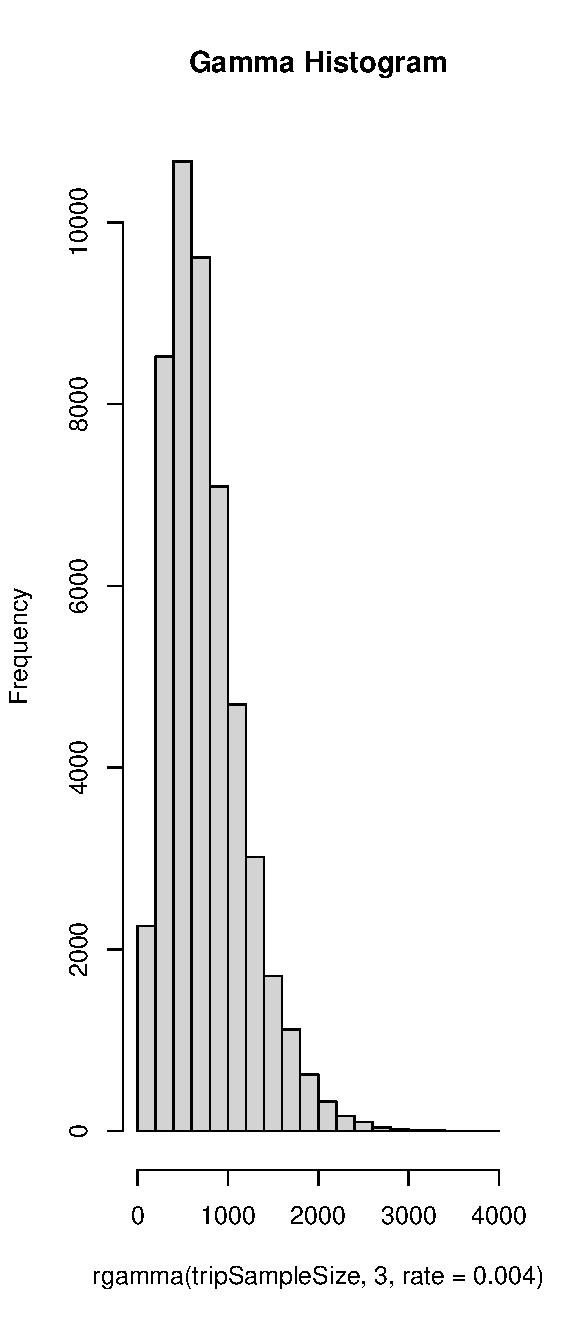
\includepdf[pages={1}]{gammas.pdf}
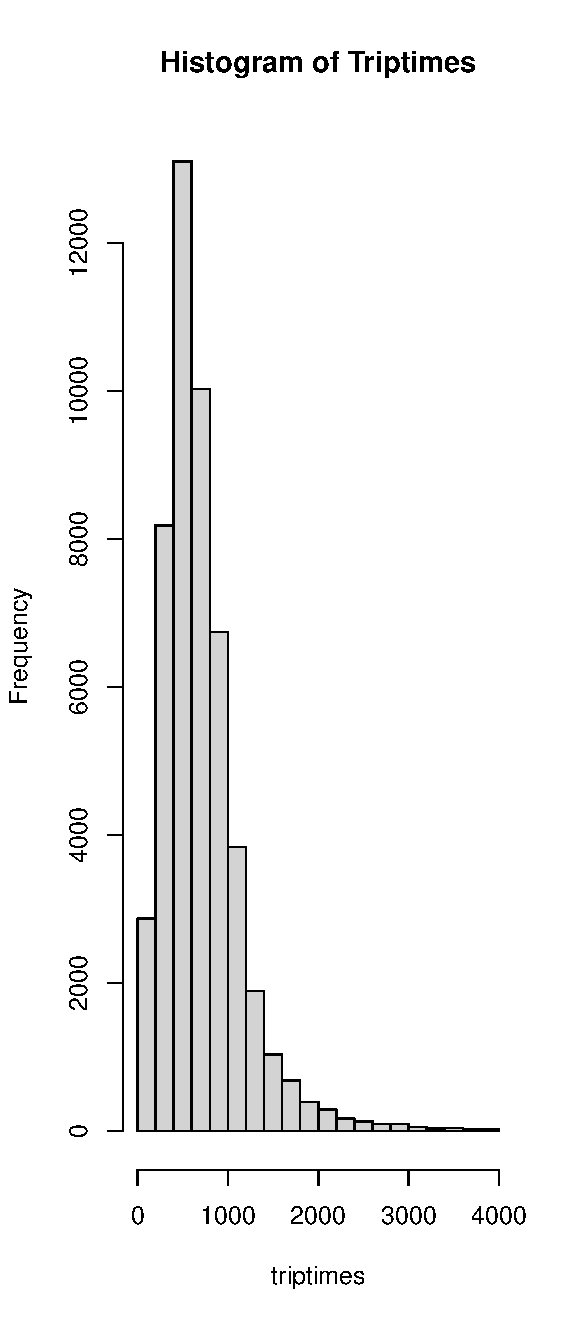
\includepdf[pages={1}]{triptimes.pdf}

% TODO add important code and figures

\section{Part B Task 2}
In this part, we are exploring a model from one of our density families that best fit B, denoting the proportion of time a driver is busy. After researching, we found that in Portugal, it is common for the work day to be divided into two periods. The first working period followed by a 2 hour break and the second working period to finish the working day. Following this line of logic, we assumed that any time that there was a duration longer than 2 hours between the end of a trip and the start of the next, it was a break and the driver was not working. This is important to distinguish because we are trying to find the proportion of time a driver is busy against the time a driver is waiting when they are actually working. This time should not include when the driver is in bed or eating dinner. To validate this assumption, we made a function to find the amount of time between the end of a trip and the start of the next for all trips for all drivers. We ran this function on all of the drivers and found the mean number of breaks that were over 2 hours for each driver.
\begin{lstlisting}[language=R]
finddifference<-function(d){ 
  workingtime <- vector()
  for(i in 2:length(d$TRIP_ID)){
    time <- length(unlist
    (strsplit(d$POLYLINE[i-1], "\\],\\["))) * 15 
    workingtime[i-1] = d$TIMESTAMP[i] - time - d$TIMESTAMP[i-1] 
  }
  return(workingtime)
}
\end{lstlisting}

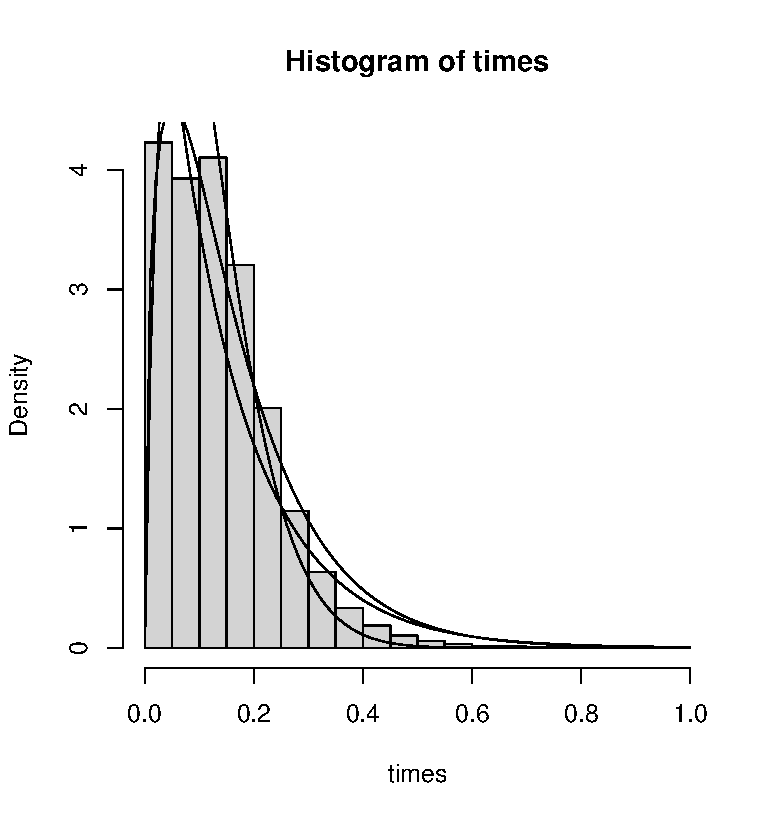
\includepdf[pages={1}]{Q2Plot.pdf}
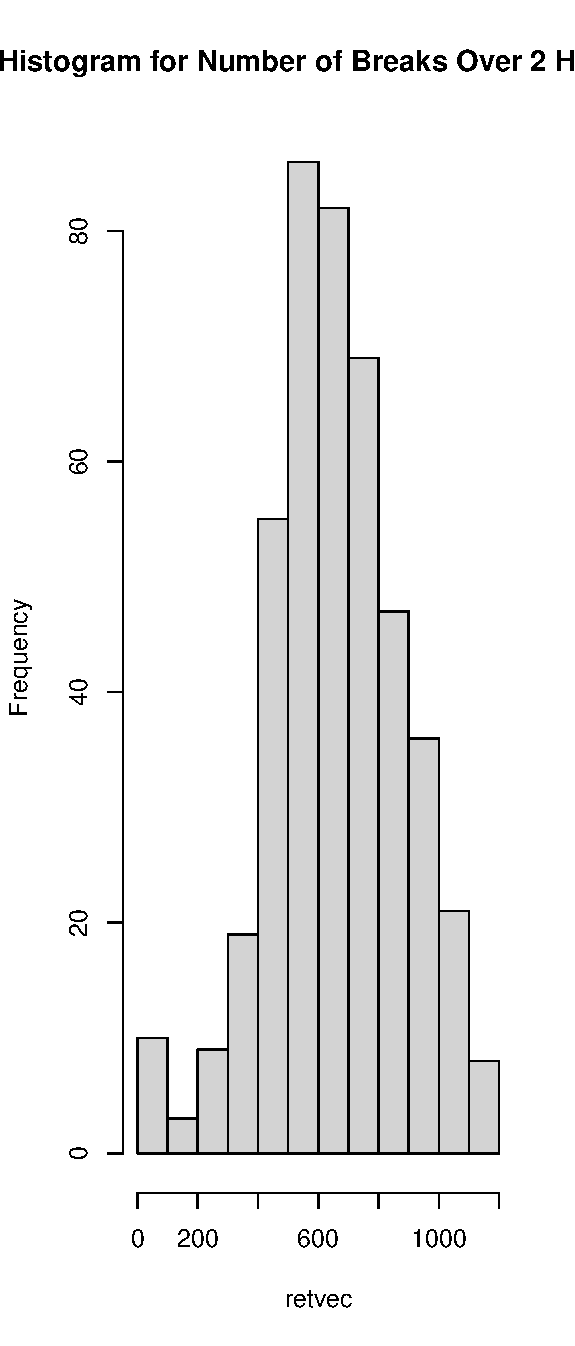
\includepdf[pages = {1}]{numbreaks.pdf}


Interestingly enough, the mean number of breaks was 656 which is nearly twice a day. This makes sense as each taxi driver would have 1 break during the day and another break once they actually stopped working. To further validate this assumption, we find the mean number of trips that each taxi driver made over the year they were tracked. This number came out to be 3818. This seems reasonable, having each driver drive 10 times a day. Now we will go through each individual taxi driver and find their proportion of working time. We ran this function on the cleaned data set from part 4. This data set has the quality of being sorted, and eliminating rows where Trip Distance is either NA or 0. We believe that these are most likely mistakes and thus not conducive to accurate statistical analysis.


Being that we are tracking a proportion where the numerator can be at most equal to the denominator, we chose to first use the beta distribution to fit our histogram. We then chose the gamma and exponential distributions. 


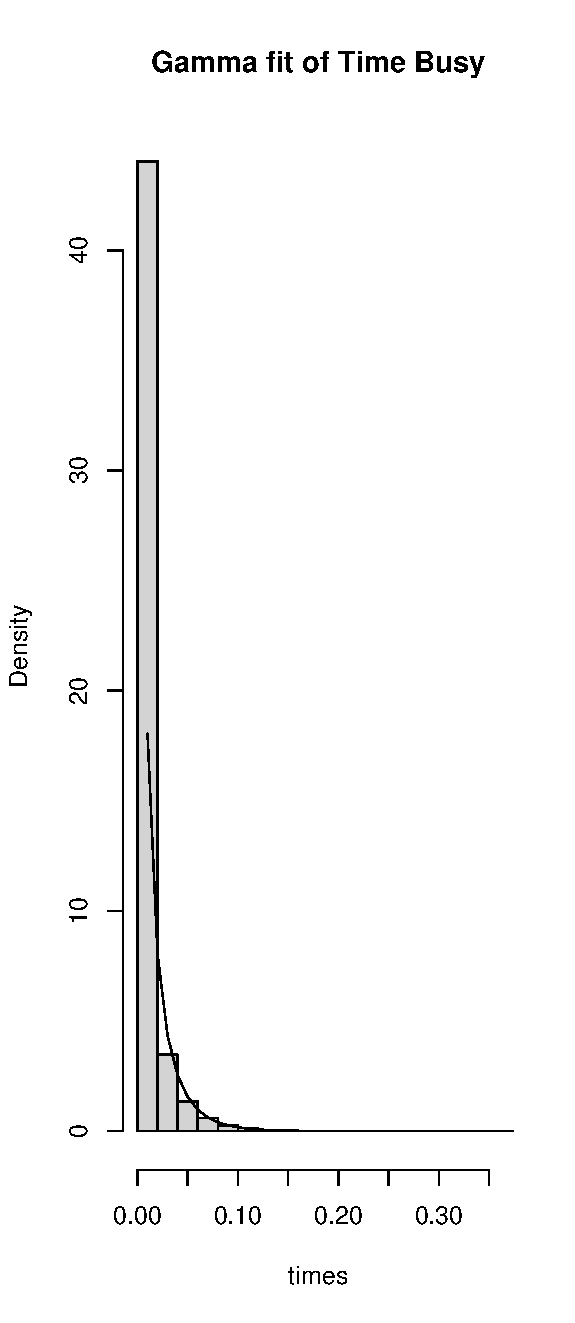
\includepdf[pages = {1}]{gamma.pdf}
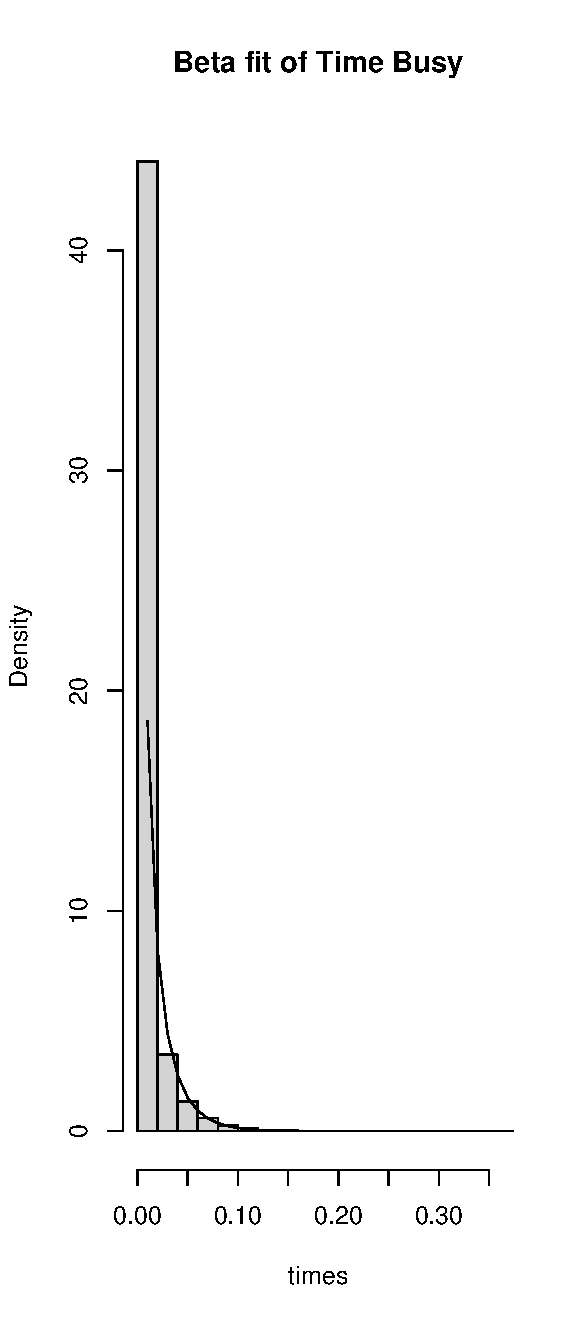
\includepdf[pages = {1}]{beta.pdf}
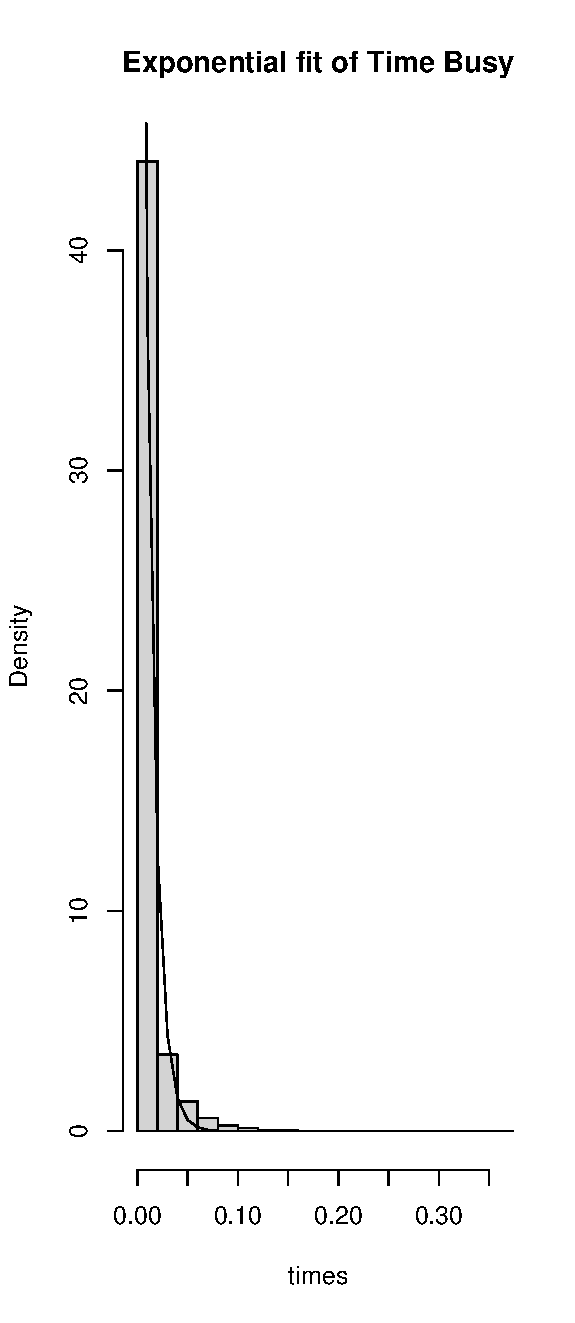
\includepdf[pages = {1}]{exponential.pdf}
Seeing how the data fits, it seems that the exponential distribution fits our random variable B best.
\section{Part B Task 3}

\indent Extrapolating data we gathered from task 1, we found that trips that were requested randomly took the longest, with a confidence interval of (784.2505, 784.4826), or about 13 minutes. We parsed data from the taxi trip data set to find the expected value, variance, coefficient of variance, and confidence intervals. Calculating the formulas for the above variables were trivial and based on what we gathered from lecture and the textbook. Using the formulas, we extracted the data from the trip call types and found interesting patterns. \\
\begin{lstlisting}[language=R]
if(strcmp("A", callType)) {
    tripTimesA <- append(tripTimesA, realTripTime)
  } else if(strcmp("B", callType)) {
    tripTimesB <- append(tripTimesB, realTripTime)
  } else if(strcmp("C", callType)) {
    tripTimesC <- append(tripTimesC, realTripTime)
  }
\end{lstlisting}

\indent The hypothesis we believe to be behind the results we got was that people using the taxi at the specific stand were more likely to visit their destination at a closer proximity, mostly likely commuting to nearby offices or tourist attractions near densely populated areas, such as downtown Porto, thus leading to a shorter duration. Furthermore, short trips in high foot traffic areas would lure customers to these taxi stands and it would make sense that there were a lot of taxi stands in these densely populated areas, where high foot traffic is inevitable. It is likely that these taxi stands would accrue customers looking for short trips at a high rate.\\
\indent To find why central dispatch and random trips were longer, individuals that could not get to taxi stands were probably more likely to be in less foot traffic areas, possibly outside the radius of the city. Assuming that most taxi customers wanted rides to popular destinations, which would be more likely to be in the center of the city, it makes sense that these individuals were located outside of the city and thus would need longer rides to get to destinations in the middle of the city. This assumes that users of the central dispatch system wanted to go towards the center of the city and these central dispatches were located on the outskirts of the city. 

\subsection{Statistics}

\begin{lstlisting}

Trips requested through central dispatch

Expected value: 767.0263
Confidence interval: (766.9338, 767.1187)
Variance: 251196.4
Coefficient of variation: 0.6534261

Trips requested from a stand

Expected value: 679.1465
Confidence interval: (679.1054, 679.1876)
Variance: 252618.9
Coefficient of variation: 0.7400643

Trips requested at random, such as on a street corner

Expected value: 784.3666
Confidence Interval: (784.2505, 784.4826)
Variance: 831774.2
Coefficient of variation: 1.162743
\end{lstlisting}


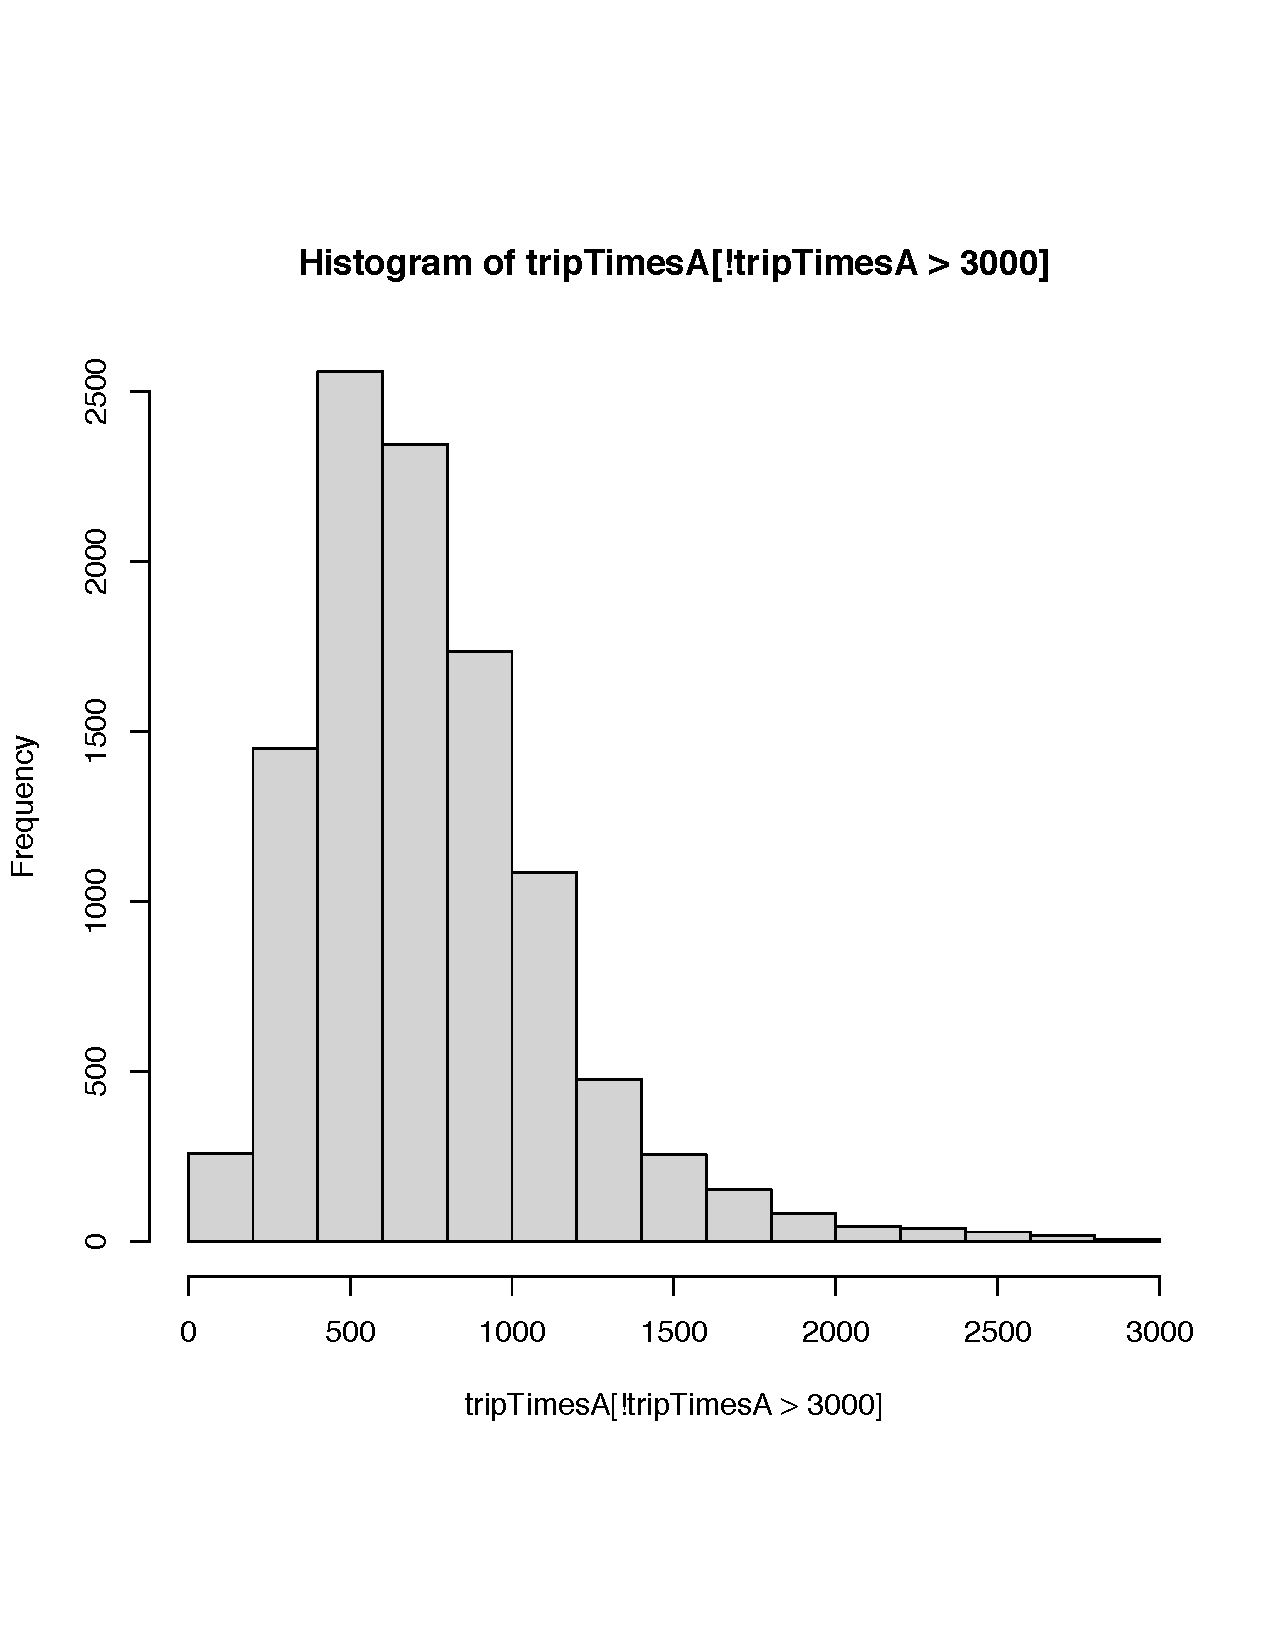
\includepdf[pages={1-3}]{PlotsOfCallType.pdf}



\section{Part B Task 4}
In this section of the project, we need to find ways to predict trip duration. There were many ways to approach this problem but we thought it best to first manipulate the data set to be more convenient for us before continuing. First, it would be nice to have a trip duration next to each trip in the data set. Second, we must find a way to get a reasonable estimate and add that estimate to each row of the data set. Finally, the data set that we were given did not have the day type properly updated. As such, our team developed functions for updating the day type according to Portugal's national holiday schedule.

One obvious problem that we ran into was the size of the data set. Running any type of manipulation would take extremely long amounts of time. We decided to take a random sample of 50000 rows as our data set. From there, we found the length and distance of each trip and added it to the data set. To find official holidays, we found holidays that would have happened during the time span of the trip, and converted the date to a UNIX time stamp. After, we fed the data set into a function that sorts the data, and goes through each day updating it to "A","B', or "C" as needed. The function is shown below:

\begin{lstlisting}[language=R]
changedays <- function(data, times){
  sorted <- data[order(data$TIMESTAMP),]
  holidays <- sort(times)
  timeinterval <- 3600 *24
  for(i in 1:length(sorted$TIMESTAMP)){
    while(sorted$TIMESTAMP[i]> (holidays[1] + timeinterval)){ 
      if(length(holidays) == 1){
        return (sorted)
      }
      holidays <- holidays[2:length(holidays)]  
    }
    if((sorted$TIMESTAMP[i] >holidays[1]- timeinterval)
    &(sorted$TIMESTAMP[i] <holidays[1])){ 
      sorted$DAY_TYPE[i] <- "C"
    }
    if(sorted$TIMESTAMP[i] > holidays[1]){
      sorted$DAY_TYPE[i] <-"B"
    }
  }
  return (sorted)
}
\end{lstlisting}
Our approach to estimating distance covered during a trip was taking the first and last coordinates in a given poly line, and finding the distance between the two. We acknowledge that finding the distance between each consecutive pair and adding up the total distance would have been more accurate but this was a trade off we were willing to take for better performance. The code for finding distance is shown below:
\begin{lstlisting}[language=R]
finddistance<- function(string){ 
  coordinates <-  unlist(strsplit(string, "\\],\\["))
  firstcoord <- coordinates[1]
  firstcoord <- unlist(strsplit(firstcoord, "\\[\\["))[2]
  pair1 <- vector()
  pair1[1]<- as.numeric(unlist(strsplit(firstcoord,","))[1])
  pair1[2]<- as.numeric(unlist(strsplit(firstcoord,","))[2])
  lastcoord <- coordinates[length(coordinates)]
  lastcoord <- unlist(strsplit(lastcoord, "\\]\\]"))[1]
  pair2 <- vector()
  pair2[1]<- as.numeric(unlist(strsplit(lastcoord,","))[1])
  pair2[2]<- as.numeric(unlist(strsplit(lastcoord,","))[2])
  return (distGeo(pair1,pair2))
  
\end{lstlisting}
Finally we tested linear models on different combinations of variables available to us. With our sample of the data set. On the linear prediction model, the model had the lowest mean absolute prediction error when just using distance as a predictor variable. This could be due to the fact that distance may have the most direct effect on time when compared to call type and day type. We also tried running on the polynomial-linear model. It's accuracy was one of the worst. This could be due to the fact that as distance goes up, there isn't a magic turning point where after a certain distance, the time to travel goes down. It's generally a positive relationship between time and distance. The linear model using distance as a predictor variable gave a mean absolute prediction error of 278.

Our group thought that using the three variables, day type, call type, and distance covered gave us a decent estimate. Our conditional expectation for a trip that was of call type c, day type A and trip distance of about 2000 to be 649 seconds. In addition, there is a 95 percent chance that the population mean for such a calculation is in between (540, 703). The bounds could have been tighter with a larger sample size but this was simply a trade off between program speed and tightness of bounds.

Finally, the two machine learning methods we used were K-nearest neighbors (KNN) and Neural Networks (NN). We used K-nearest-neighbors to predict trip duration and distance based on the closest number of trips in duration and proximity in the taxi trip data. To use KNN, we used euclidean geometry within R to find the smallest distances and calculated predictions based on the smallest distances. Neural networks consist of many layers, and within these layers, there are many nodes. Each of these layers have outputs as linear combinations of the same amount of nodes within those layers. The outputs of the first layer will then be inputted into the second layer, and then you can see the pattern from there. In regards to regression analysis, the outputs of the last layer will be averaged together to produce an estimated prediction model. Interestingly enough, changing the number of neighbors for the KNN model from 25 to 30, and finally to 28 gave increasingly better results. Our mean absolute prediction error from this model was 263 when using 28 neighbors. We found that decreasing the number to 15, or 100 allowed too narrow or too broad a spectrum of data points to affect the outcome of our model.

In regards to Neural Networks, we first tried using all predictor variables available to us. The result was a mean absolute prediction error of 400. This could be due to over fitting. When using only distance, we were able to reduce the error to 287.

Overall, in terms of predictive power, when all models are optimized, it seems that the predictive powers are quite similar. These results could have easily had Neural Networks or K nearest neighbors as the most accurate model had the sample randomly chosen more favorable rows. One common theme represented across all models is the lack of need for excessive information. It seemed that most models did worse when including day type indicating that day type had no clear correlation with trip duration in our sample. In contrast, using fewer variables often led to more accurate results. To validate this, we ran qeCompare() on the four models used using only distance as a predictor variable 25 times. The results are as follows: -qeLin 296.0226 -qePolyLin 347.5958 -qeKNN 291.8229 -qeNeural 294.6121
\section{Contributions}
Nathan- Nathan worked on fitting our densities to the portion of time a taxi driver was busy and worked on predicting trip time based on predictor variables. He also updated the data set to have correct day types, and to include trip time and duration to make modeling easier. He also worked on translating the fitting and prediction parts to latex. He wrote the code for part 2 and part 4.
Derek-Derek worked on attempting to find models for trip duration and possible density families. He also worked on coming up with explanations for why certain call types had different duration than other call types. Attempted machine learning methods and linear modeling.
Grayson-Grayson wrote the code for parts 1 and 3, and worked on the individual portion as well. This included finding an appropriate paper, determining the average trip time, matching it with a distribution (gamma) and split up the trip times by call type and wrote the statistics/graphing  portions to determine how call type affects those statistics
\section{Appendix}
\begin{lstlisting}[language=R]
tripSampleSize <- 50000
hist(rgamma(tripSampleSize, 3, rate=.004),  main = "Gamma Histogram")
porto.data <- read.csv("C://Users/natha/Downloads/train.csv/train.csv") #make sure that this is right for your computer
triptimes <- c()
for(i in sample(1:length(porto.data$POLYLINE), tripSampleSize, replace=TRUE)) {
  triptime <- as.numeric(lapply(strsplit(porto.data$POLYLINE[i], "\\],\\["), length)) 
  #print((triptime * 15)/60) 
  if(triptime * 15 < 4000) {
    triptimes <- append(triptimes, triptime * 15)
  }
}
hist(triptimes, main = "Histogram of Triptimes")
#PART B
#FUNCTIONS:
truncated <- porto.data[sample(nrow(porto.data), 50000),]
for(i in 1:length(truncated$POLYLINE)){
  truncated$TRIPDURATION[i] <- length(unlist(strsplit(truncated$POLYLINE[i], "\\],\\["))) * 15
  truncated$TRIPDISTANCE[i] <- finddistance(truncated$POLYLINE[i])
}
#Now lets clean the data
cleaned <- truncated[complete.cases(truncated$TRIPDISTANCE),] # we don't want na values, or values that are zero
cleaned <- cleaned[cleaned$TRIPDISTANCE!=0,] #it means that a trip didn't happen, or only one pair which is 15 seconds. Most likely a mistake

finddifference<-function(d){ #function finds the time between trips for all trips
  workingtime <- vector()
  for(i in 2:length(d$TRIP_ID)){ # for every pair
    time <- length(unlist(strsplit(d$POLYLINE[i-1], "\\],\\["))) * 15 # take the amount of pairs and multiply by 15
    workingtime[i-1] = d$TIMESTAMP[i] - time - d$TIMESTAMP[i-1] # add to previous time stamp, and subtract from current to find break
  }
  return(workingtime)
}

findworkingtime <-function(d){
  timedriving <- 0
  timeworking <- 0
  index <- 1
  breakoff_time <- 2* 3600
  #If the period between the end of the last trip and the beginning of the next
  #is greater than 2 hours, we can assume that the taxi driver has stopped working
  f<- list()
  for(i in 2:length(d$TIMESTAMP)){
    time <- length(unlist(strsplit(d$POLYLINE[i], "\\],\\["))) * 15 
    timedriving <- timedriving + time 
    # Driver is currently working, he has actively driven for time amount
    # So we add it to timedriving
    if((d$TIMESTAMP[i] - time - d$TIMESTAMP[i-1]) > breakoff_time){ 
      #The driver has not been driving for at least 2 hours.
      #The total time period is the previous timestamp + time just driven
      #subtracted from the beginning of the working period.
      f[length(f) + 1] <- timedriving/(time + d$TIMESTAMP[i] - d$TIMESTAMP[index])# the index is where our period starts
      index <- i #new working period starts at the current timestamp
      timedriving <-0 #reset timedriving
    }
  }
  return (f)
}
# The amount of breaks has few outliers. Lets see if we can explain it.
#In Portugal, it is common for breaks to be 2 hours.

retvec <-vector()
for(i in 1:length(unique(porto.data$TAXI_ID))){ # go through each taxi, and find the amount of working time
  newdata <- porto.data[porto.data$TAXI_ID == unique(porto.data$TAXI_ID)[i],]
  retvec[i] <- sum(finddifference(newdata) > 7200) # find number of breaks for each taxi that are above 7200
}
mean(retvec, na.rm = TRUE)
hist(retvec, main = "Histogram for Number of Breaks Over 2 Hours")
# The mean number of breaks for all taxi drivers over 2 hours
#is 656.9056, nearly twice a day. This makes sense because the drivers will
#take one break, and one longer break once they actually stop working. (go home)
# to find number of trips on average to validate above assumption
numtrips <- vector()
for(i in 1:length(unique(cleaned$TAXI_ID))){
  newid <- unique(cleaned$TAXI_ID)[i]
  newdata <- cleaned[mydata$TAXI_ID == unique(cleaned$TAXI_ID)[i],]
  numtrips[i] <- length(newdata$TRIP_ID)
}
mean(numtrips)
# The mean number of trips was 3818. This is reasonable. Most of the drivers
#are driving around 10 times a day.

times <- vector()
#we are using dataset cleaned which is the cleaned version of mydata. The cleaning was done in p4.r.
for(i in 1:length(unique(cleaned$TAXI_ID))){
  newdata <- cleaned[cleaned$TAXI_ID == unique(cleaned$TAXI_ID)[i],]
  c<-findworkingtime(newdata)
  times[(length(times)+1):(length(times) + length(c))] <- unlist(c)
}
estBetaParams <- function(mu, var) {
  alpha <- ((1 - mu) / var - 1 / mu) * mu ^ 2
  beta <- alpha * (1 / mu - 1)
  return(params = list(alpha = alpha, beta = beta))
}
# https://stats.stackexchange.com/questions/12232/calculating-the-parameters-of-a-beta-distribution-using-the-mean-and-variance

betaparams<- estBetaParams(mean(times[times<1], rm.na = TRUE), (var(times[times<1])))
gamma1<- mean(times[times<1], rm.na = TRUE)^2/var(times[times<1])
gamma2<- mean(times[times<1], rm.na = TRUE)/var(times[times<1])
hist(times, main = "Gamma fit of Time Busy",freq = FALSE)
curve(dgamma(x,betaparams$alpha,betaparams$beta),0,1, add= TRUE)
hist(times, main = "Beta fit of Time Busy", freq = FALSE)
curve(dbeta(x,gamma1,gamma2),0,1, add= TRUE)
hist(times, main = "Exponential fit of Time Busy",freq = FALSE)
curve(dexp(x,1/mean(times[times<1], rm.na = TRUE)), 0,1,add = TRUE)
#The exponential distribution seems to be the best fit.
mean(times, rm.na = TRUE)
mean(times[times<1], rm.na = TRUE)

#PART C
expectedValue <- function(values) {
  return(sum(values) / length(values))
}

variance <- function(values) {
  return(expectedValue(values ^ 2) - expectedValue(values) ^ 2)
}

coefficientOfVariation <- function(values) {
  return(sqrt(variance(values)) / expectedValue(values))
}

standardDeviation <- function(values) {
  return(sqrt(variance(values)/length(values)))
}

confidenceInterval95 <- function(values) {
  marginOfError <- 1.96 * standardDeviation(values) / sqrt(length(values))
  conInt <- c(expectedValue(values) - marginOfError, expectedValue(values) + marginOfError)
  return(conInt)
}

printStats <- function(tripTimesA, tripTimesB, tripTimesC) {
  expectedValueA <- expectedValue(tripTimesA)
  expectedValueB <- expectedValue(tripTimesB)
  expectedValueC <- expectedValue(tripTimesC)
  
  confidenceIntervalA <- confidenceInterval95(tripTimesA)
  confidenceIntervalB <- confidenceInterval95(tripTimesB)
  confidenceIntervalC <- confidenceInterval95(tripTimesC)
  
  varianceA <- variance(tripTimesA)
  varianceB <- variance(tripTimesB)
  varianceC <- variance(tripTimesC)
  
  coefficientOfVariationA <- coefficientOfVariation(tripTimesA)
  coefficientOfVariationB <- coefficientOfVariation(tripTimesB)
  coefficientOfVariationC <- coefficientOfVariation(tripTimesC)
  
  print("Trips requested through central dispatch")
  print("Expected value")
  print(expectedValueA)
  print("Confidence interval")
  print(confidenceIntervalA)
  print("Variance")
  print(varianceA)
  print("Cooefficient of variation")
  print(coefficientOfVariationA)
  
  print("Trips requested from a stand")
  print("Expected value")
  print(expectedValueB)
  print("Confidence interval")
  print(confidenceIntervalB)
  print("Variance")
  print(varianceB)
  print("Cooefficient of variation")
  print(coefficientOfVariationB)
  
  print("Trips requested at random, such as on a street corner")
  print("Expected value")
  print(expectedValueC)
  print("Confidence Interval")
  print(confidenceIntervalC)
  print("Variance")
  print(varianceC)
  print("Cooefficient of variation")
  print(coefficientOfVariationC)
}

tripSampleSize <- 50000
tripTimesA <- c() # Dispatch from central
tripTimesB <- c() # Trip requested from stand
tripTimesC <- c() # Trip requested randomly, such as on a street
for(i in sample(1:length(porto.data$POLYLINE), tripSampleSize, replace=TRUE)) {
  beacons <- as.numeric(lapply(strsplit(porto.data$POLYLINE[i], "\\],\\["), length)) 
  realTripTime <- beacons * 15
  callType <- porto.data$CALL_TYPE[i]
  
  if(strcmp("A", callType)) {
    tripTimesA <- append(tripTimesA, realTripTime)
  } else if(strcmp("B", callType)) {
    tripTimesB <- append(tripTimesB, realTripTime)
  } else if(strcmp("C", callType)) {
    tripTimesC <- append(tripTimesC, realTripTime)
  }
}

printStats(tripTimesA, tripTimesB, tripTimesC)

hist(tripTimesA)
hist(tripTimesB)
hist(tripTimesC)

#PART D

finddistance<- function(string){ #this function just needs the polyline, we will then strip away the first two brackets, and last two brackets on the first
  #and last element respectively.
  coordinates <-  unlist(strsplit(string, "\\],\\["))
  firstcoord <- coordinates[1]
  firstcoord <- unlist(strsplit(firstcoord, "\\[\\["))[2]
  pair1 <- vector()
  pair1[1]<- as.numeric(unlist(strsplit(firstcoord,","))[1])
  pair1[2]<- as.numeric(unlist(strsplit(firstcoord,","))[2])
  lastcoord <- coordinates[length(coordinates)]
  lastcoord <- unlist(strsplit(lastcoord, "\\]\\]"))[1]
  pair2 <- vector()
  pair2[1]<- as.numeric(unlist(strsplit(lastcoord,","))[1])
  pair2[2]<- as.numeric(unlist(strsplit(lastcoord,","))[2])
  return (distGeo(pair1,pair2))
  
}

changedays <- function(data, times){
  sorted <- data[order(data$TIMESTAMP),] # need to sort by timestamp for the below logic to work
  holidays <- sort(times)
  timeinterval <- 3600 *24
  for(i in 1:length(sorted$TIMESTAMP)){
    while(sorted$TIMESTAMP[i]> (holidays[1] + timeinterval)){ # we have already sorted the times, so if we are greater than the current holiday, we dont' need to worry about
      if(length(holidays) == 1){ # it anymore
        return (sorted)
      }
      holidays <- holidays[2:length(holidays)]  
    }
    if((sorted$TIMESTAMP[i] >holidays[1]- timeinterval) &(sorted$TIMESTAMP[i] <holidays[1])){ # if it is 24 hours before holiday
      sorted$DAY_TYPE[i] <- "C"
    }
    if(sorted$TIMESTAMP[i] > holidays[1]){ # we know that if it is greater than the holiday, it is not by more than 24 hours
      sorted$DAY_TYPE[i] <-"B"
    }
  }
  return (sorted)
}
# TASK A and B have been taken care of in the second part of the project.
#TASK C
# We need to fix the data as the day types are incorrect
# Use an online unix time to date converter to find holidays and change the days  
#Below are the unix timestamps for Portugal's holidays from 2013 - 2014
holidays <- vector()
holidays[1] <-1401778800
holidays[2] <-1402383600
holidays[3] <- 1402642800
holidays[4] <- 1376550000
holidays[5] <- 1380956400
holidays[6] <- 1383289200
holidays[7] <- 1385884800
holidays[8] <- 1386489600
holidays[9] <- 1387958400
holidays[10] <- 1388563200
holidays[11] <- 1392364800
holidays[12]<-1392451200
holidays[13] <-1396422000
holidays[14] <-1396594800
holidays[15] <-1396681200
holidays[16]<-1398409200
holidays[17] <-1398927600
holidays[18]<-1399014000
holidays[19] <-1399964400

cleaned<- changedays(cleaned, holidays)

#TASK D
# Test linear model
#Try to see Trip Duration from distance, daytype, and call type
callandday <- cleaned[, c(2,7,10,11)]
lin <- qeLin(callandday ,'TRIPDURATION')
print("Mean Absolute Prediction Error from distance, daytype, and call type.")
print(lin$testAcc)
# from distance and daytype
callandday <- cleaned[, c(7,10,11)]
lin <- qeLin(callandday ,'TRIPDURATION')
print("Mean Absolute Prediction Error from distance and daytype.")
print(lin$testAcc)
#from distance and call type
callandday <- cleaned[, c(2,10,11)]
lin <- qeLin(callandday ,'TRIPDURATION')
print("Mean Absolute Prediction Error from distance and call type.")
print(lin$testAcc)
#from calltype and daytype
callandday <- cleaned[, c(2,7,10)]
lin <- qeLin(callandday ,'TRIPDURATION')
print("Mean Absolute Prediction Error from daytype, and call type.")
print(lin$testAcc)
#from distance
callandday <- cleaned[, c(10,11)]
lin <- qeLin(callandday ,'TRIPDURATION')
print("Mean Absolute Prediction Error from distance")
print(lin$testAcc)
#from calltype
callandday <- cleaned[, c(2,10)]
lin <- qeLin(callandday ,'TRIPDURATION')
print("Mean Absolute Prediction Error from call type.")
print(lin$testAcc)
#from daytype
callandday <- cleaned[, c(7,10)]
lin <- qeLin(callandday ,'TRIPDURATION')
print("Mean Absolute Prediction Error from daytype.")
print(lin$testAcc)
#Trying polylin on the distance
callandday <- cleaned[, c(10,11)]
lin <- qePolyLin(callandday ,'TRIPDURATION')
print("Mean Absolute Prediction Error from distance using polylin.")
print(lin$testAcc)
#it seems using all three variables as predictors gives us a reasonable error so lets use that as our model
#set arbitrary u calltype = c, daytype = a, distance = 2000
#having a strict bearing on distance being 2000 is quite useless
#so let's get the values 
#create a new set conditional that will have the above qualities
conditional <- cleaned[cleaned$CALL_TYPE == "C",]
conditional <- conditional[conditional$DAY_TYPE == "A",]
conditional <- conditional[(conditional$TRIPDISTANCE >=(.99*2000)) &(conditional$TRIPDISTANCE <= (1.01*2000)),]
mean(conditional$TRIPDURATION)
#mean trip duration was 649.5056
s2<- var(conditional$TRIPDURATION)
tail <- -qnorm(.05/2)
plusminus <- tail * sqrt(s2/length(conditional$TRIPDURATION))
confidenceinterval <- c(avgtrip - plusminus, avgtrip + plusminus)
print(confidenceinterval)
#95 % chance that values are in between (540, 703)
#if we had a larger sample size we could have much tighter bounds
#but this is simply a tradeoff between time and the tightness of our CI
#Trying machine learning methods
#Let's try K-Nearest Neighbors
#First we need to subfactor DAY_TYPE and CALL_TYPE
callandday <- cleaned[, c(2,5,7,10,11)]
callandday$DAY_TYPE <- toSubFactor(callandday$DAY_TYPE, c("A", "B"))
callandday$CALL_TYPE <- toSubFactor(callandday$CALL_TYPE, c("A", "B"))
lin <- qeKNN(callandday ,'TRIPDURATION')
print(lin$testAcc)
#Testing Error was 320
#Try only using call type and distance
callanddistance <- callandday[, c(1,4,5)]
lin <- qeKNN(callanddistance, "TRIPDURATION")
print(lin$testAcc)
#Error at 275
#Try only using distance
distanceonly <- callandday[, c(4,5)]
lin <- qeKNN(distanceonly, "TRIPDURATION")
print(lin$testAcc)
# Error at 277
#Lets take the most accurate KNN and adjust hyperparameters.
lin <- qeKNN(callanddistance, "TRIPDURATION", k=15)
print("Mean absolute prediction error for k =  15:")
print(lin$testAcc)
#Error- 288
lin <- qeKNN(callanddistance, "TRIPDURATION", k=50)
print("Mean absolute prediction error for k =  50:")
print(lin$testAcc)
#Error- 287
lin <- qeKNN(callanddistance, "TRIPDURATION", k=100)
print("Mean absolute prediction error for k =  100:")
print(lin$testAcc)
#Error- 300.5
lin <- qeKNN(callanddistance, "TRIPDURATION", k=30)
print("Mean absolute prediction error for k =  30:")
print(lin$testAcc)
#Error- 266
lin <- qeKNN(callanddistance, "TRIPDURATION", k=28)
print("Mean absolute prediction error for k =  28:")
print(lin$testAcc)
#Error- 263! Lowest one yet
#Try using Neural Networks

lin <- qeNeural(callandday ,'TRIPDURATION')
print("Mean absolute prediction error using all predictor variables")
print(lin$testAcc)
#When using all predictors, we have an error of 400! Overfitting?
lin <- qeNeural(callanddistance, "TRIPDURATION")
print("Mean absolute prediction error using call type and distance")
print(lin$testAcc)
#Only using calltype and distance, we have an error of 298.
lin <- qeNeural(distanceonly, "TRIPDURATION")
print("Mean absolute prediction error only using distance")
print(lin$testAcc)
#Only using distance we have an error of 287,
qeCompare(cleaned[, c(10,11)], "TRIPDURATION", c('qeLin', 'qePolyLin', 'qeKNN', 'qeNeural'), 25 )
\end{lstlisting}
\end{document}
